\section{Visite de Tenneville}
\subsection{Informations générales}
Dans le cadre de notre projet, nous avons visité des usines afin de collecter diverses informations.
Nous parlerons ici de l'usine de bio-méthanisation de Tenneville.
Le centre de bio-méthanisation de Tenneville est une intercommunale pour le développement de la commune du Luxembourg.
Elle traite plus de \unit{3000}{tonnes} de déchets de cuisine par an et \unit{39000}{tonnes} de déchets verts.
\subsection{Processus}
\begin{figure}
  \centering
  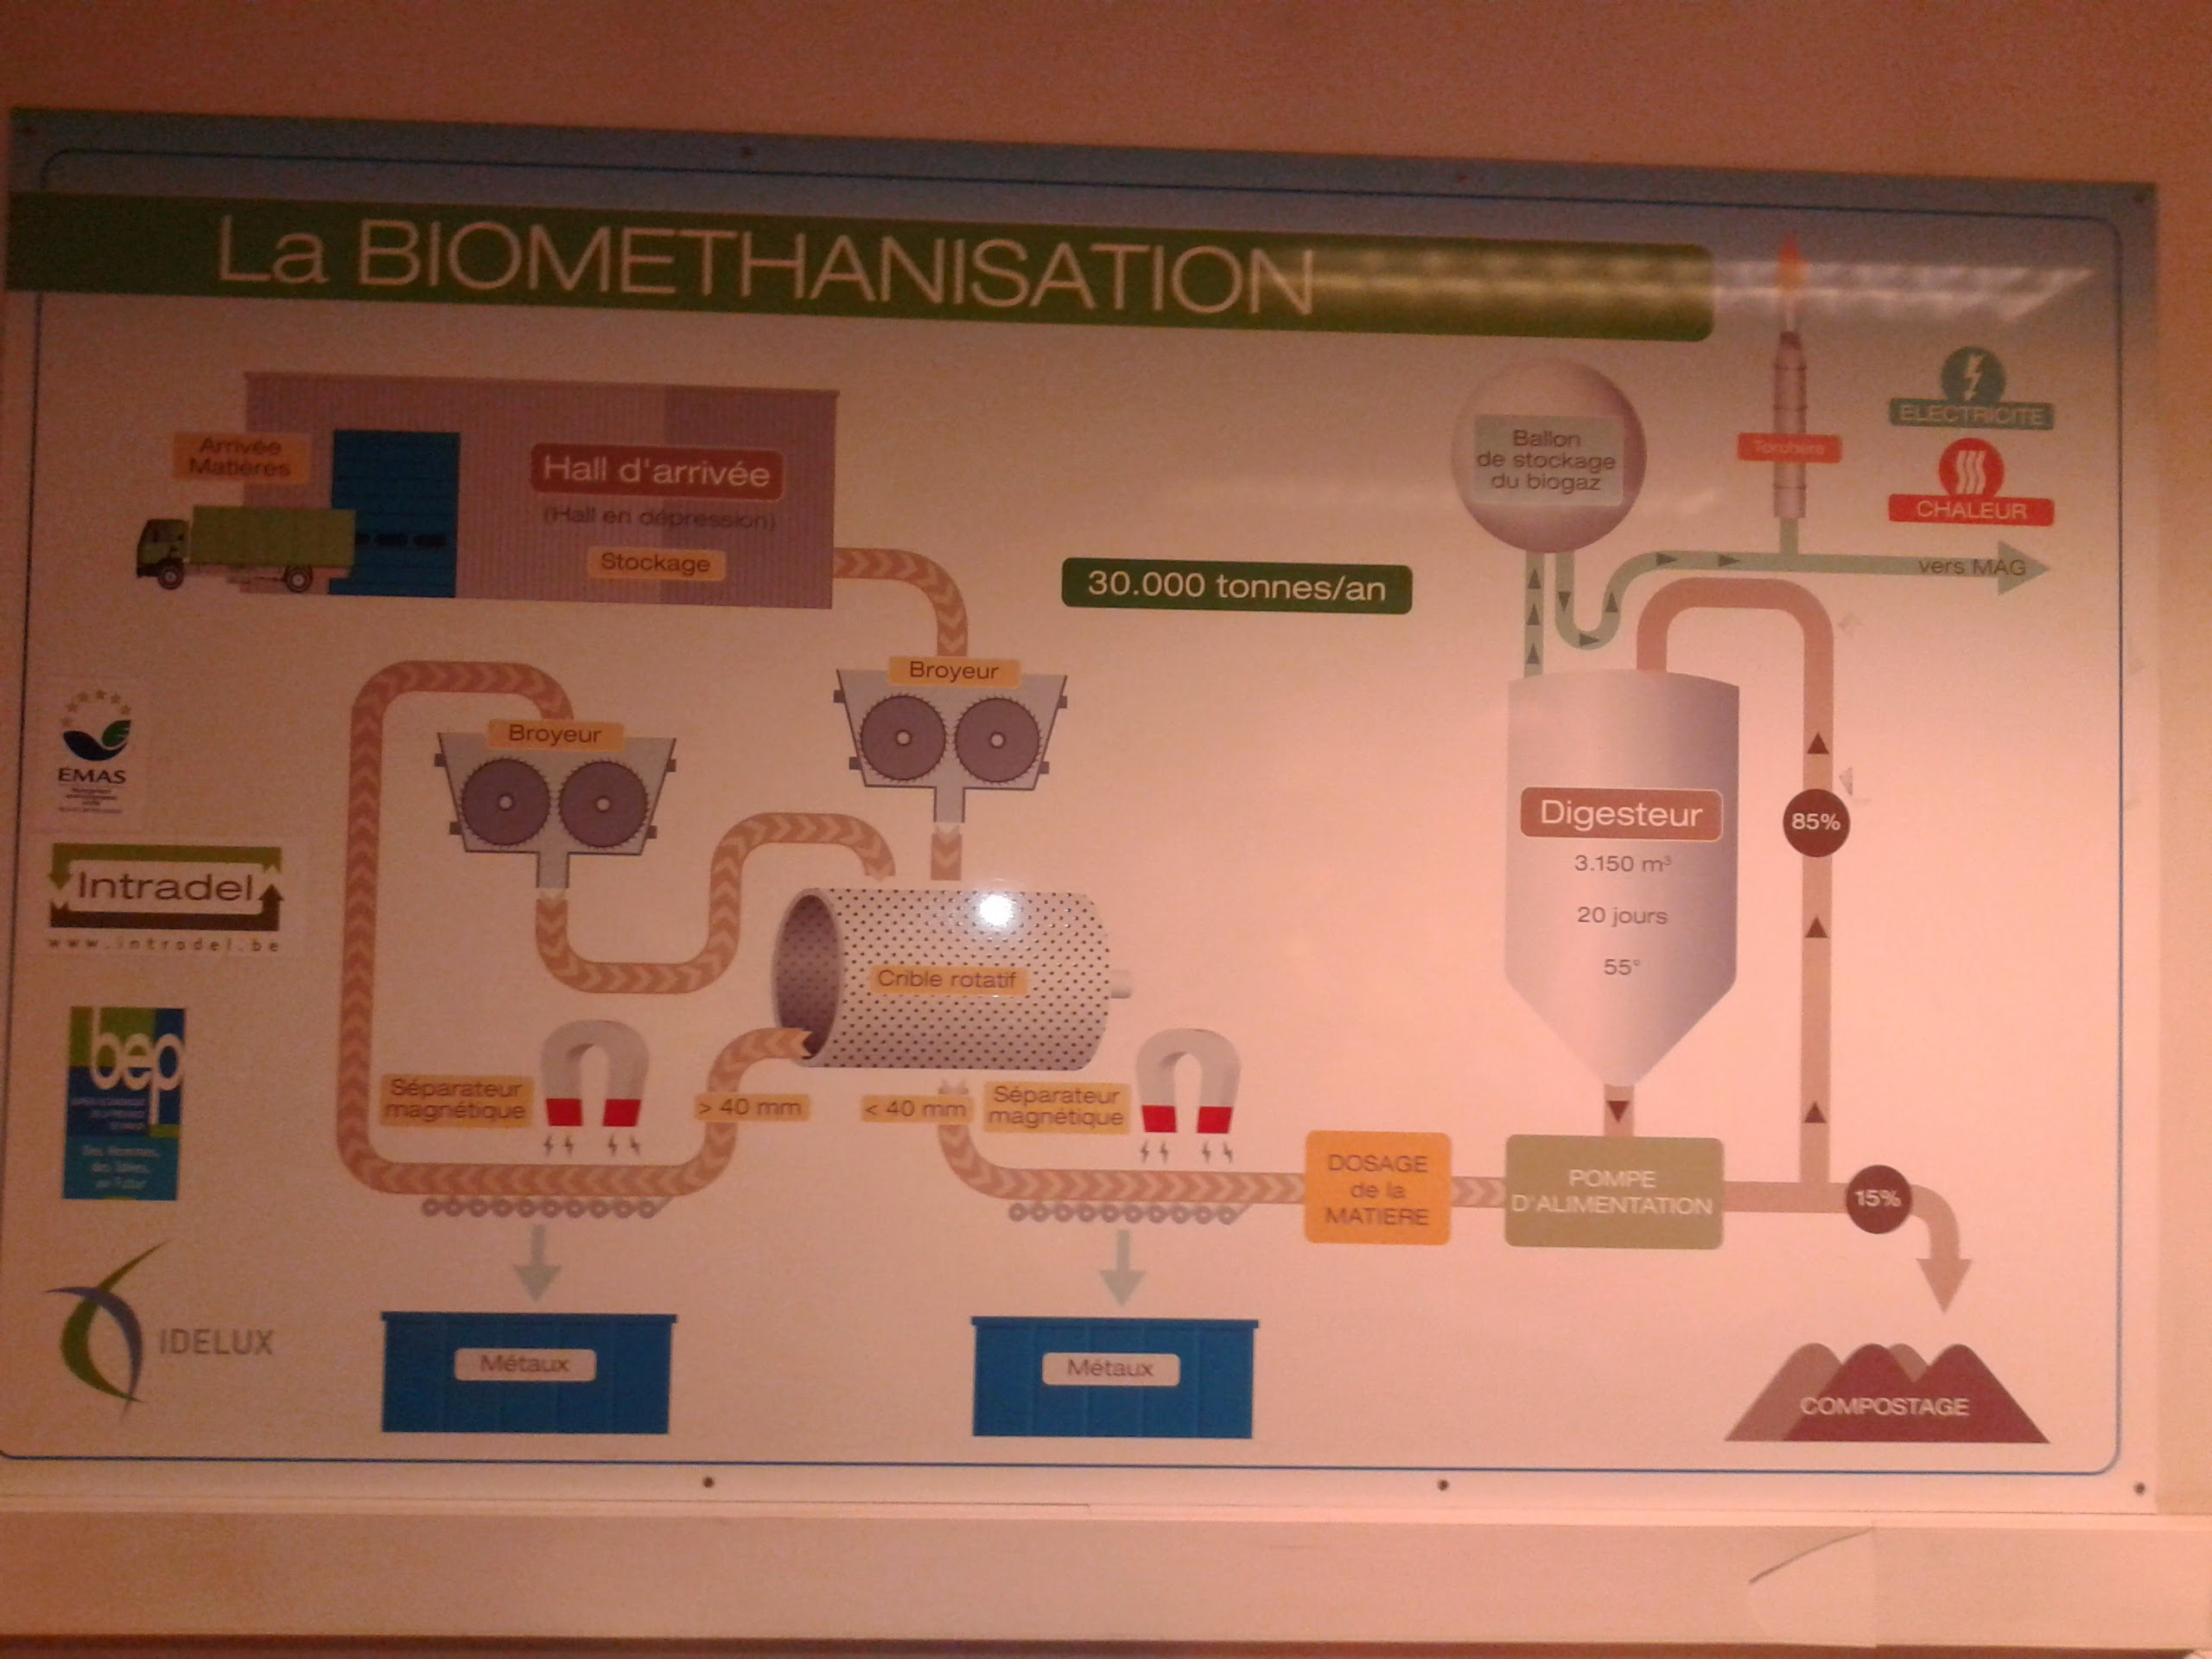
\includegraphics[scale=0.07]{task7/tenneville/IMG_20141105_105627.jpg}
  \caption{bio-méthanisation}
  \label{fig:biomethanisation}
\end{figure}
\subsubsection{Collecte des déchets}
Le centre de Tenneville récolte les déchets organiques de cuisine de plusieurs communes ainsi que tous les déchets ménagers de la commune du Luxembourg (\unit{240}{tonnes/an}). Elle collecte aussi les déchets verts et les PMC qui eux seront envoyés dans d'autres centres de tri.
A leur arrivée, les déchets de cuisine sont malheureusement pollués par, entre autre, des plastiques  et des métaux. Afin d'éliminer ces indésirables, les déchets passent dans un premier broyeur et les métaux sont récupérés grâce à un grand aimant (figure~\ref{fig:biomethanisation}). 
\subsubsection{Digesteur}
\begin{figure}
  \centering
  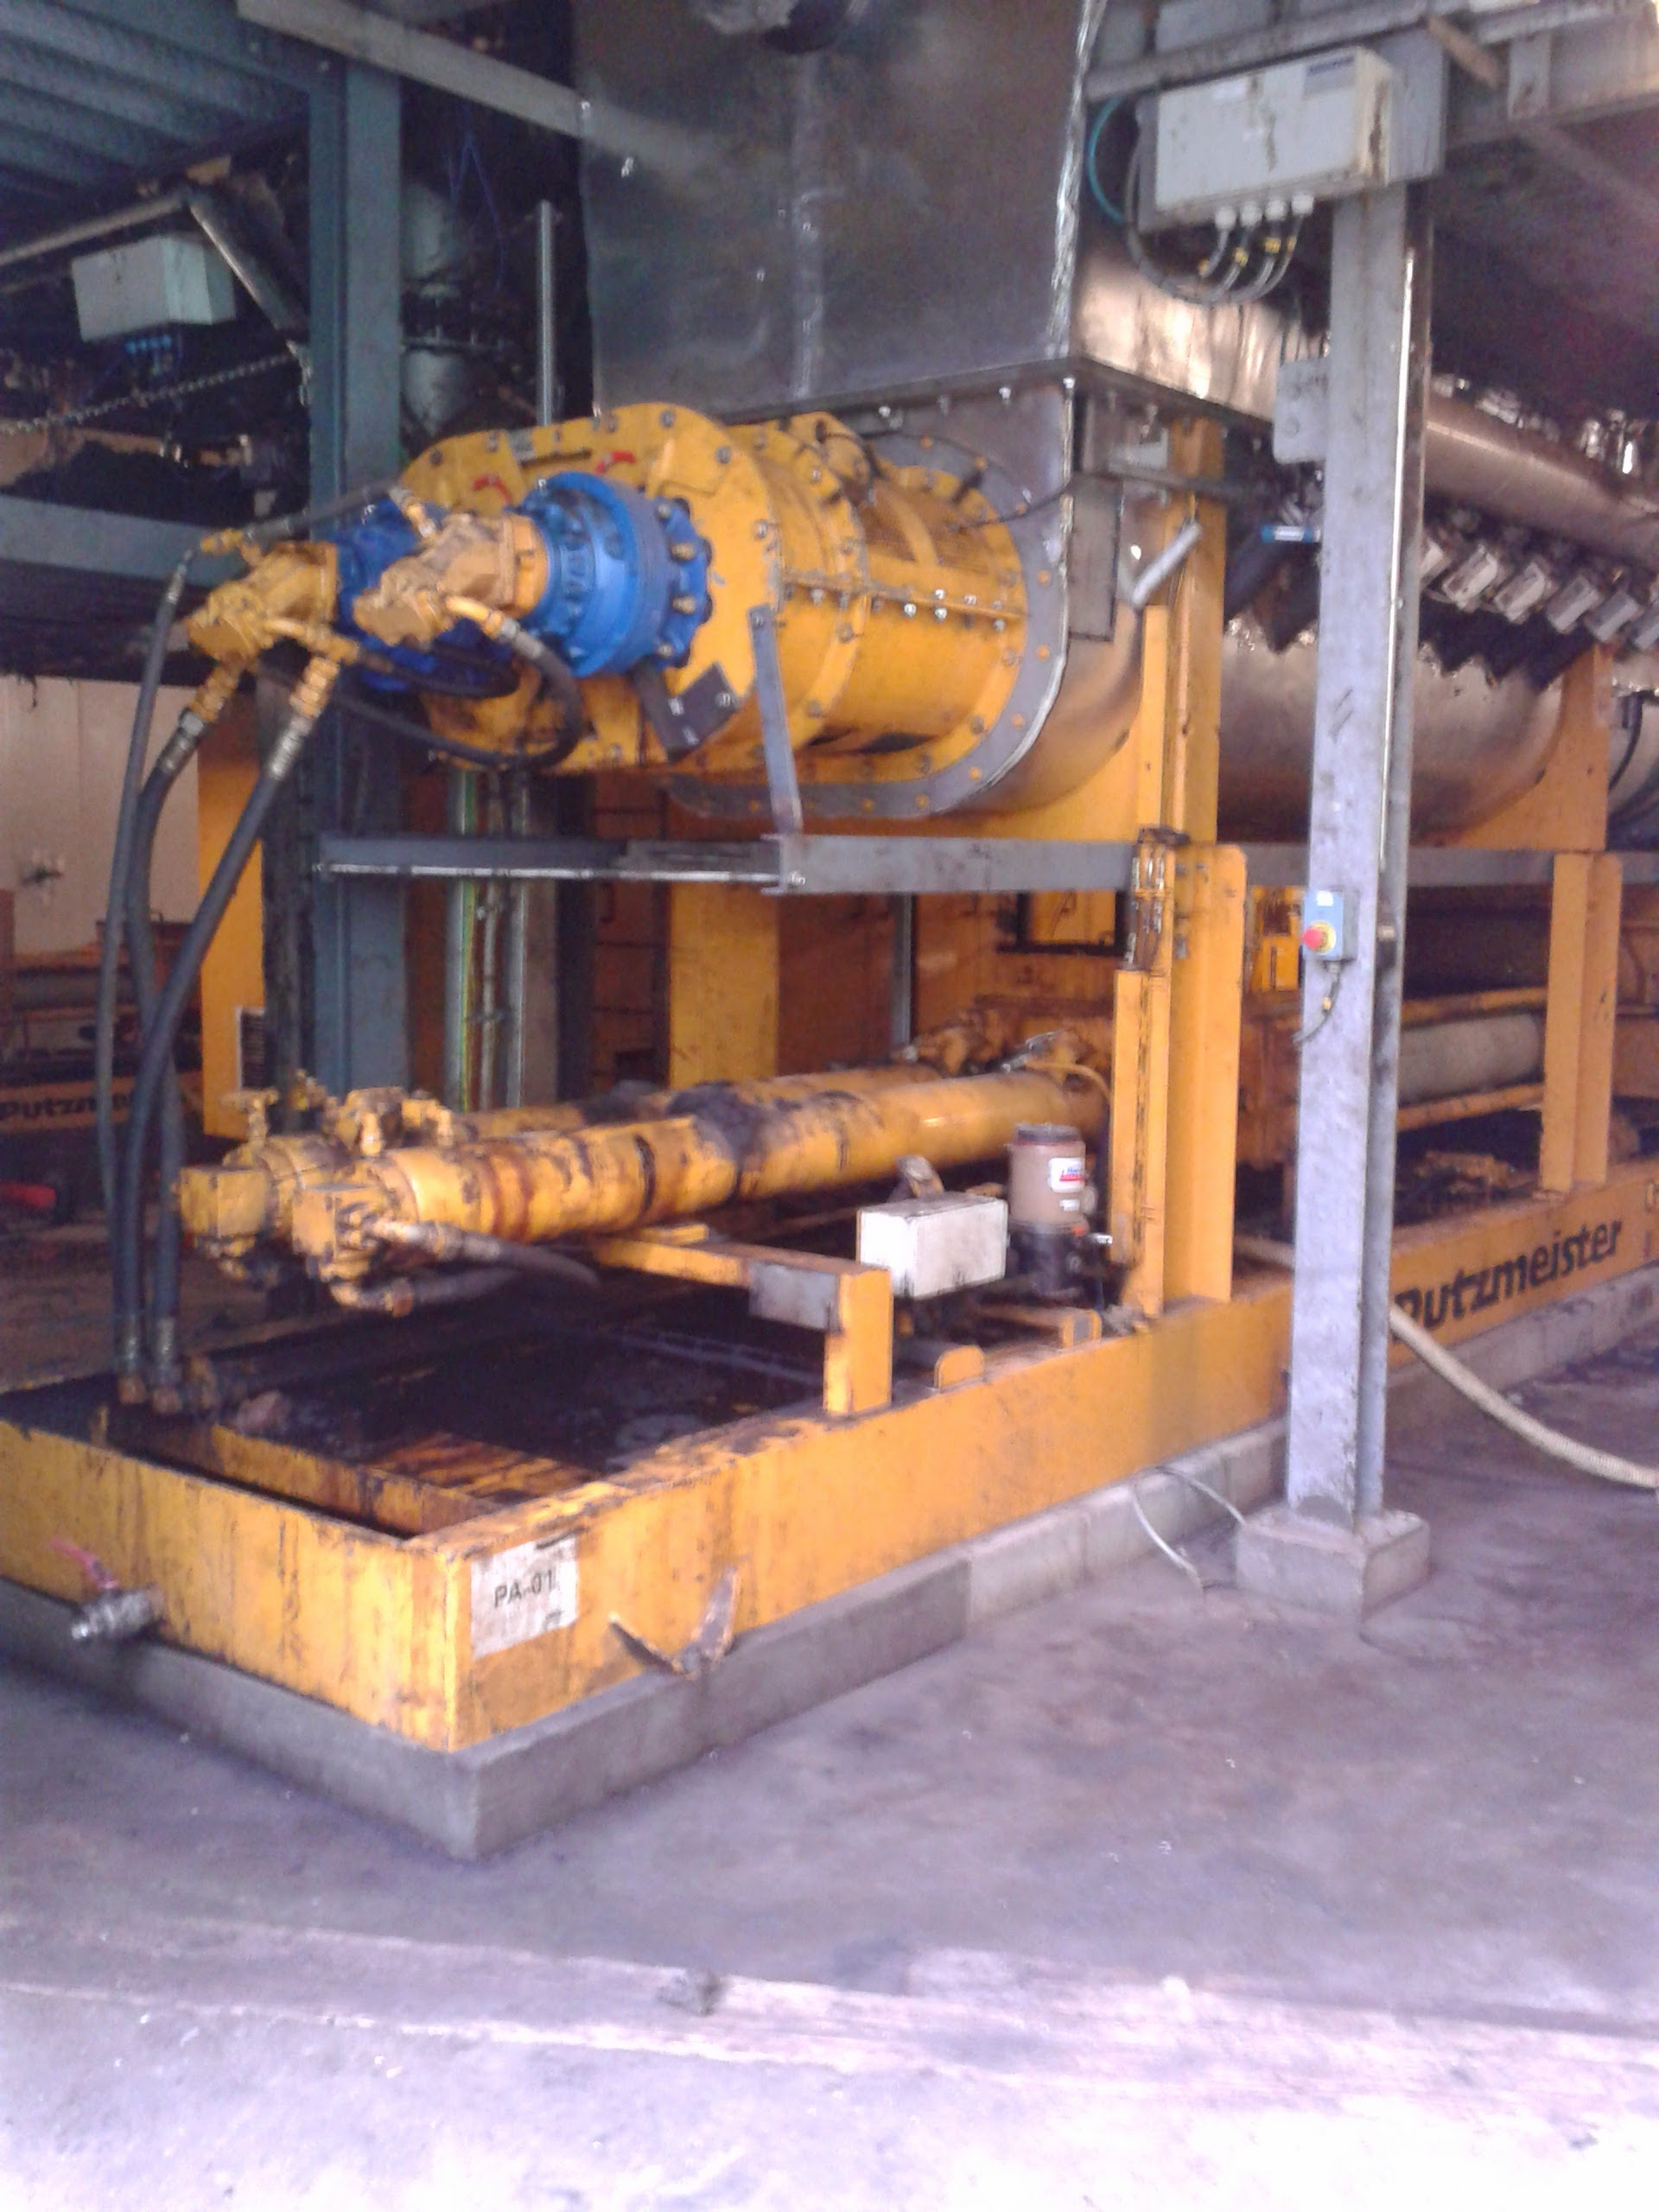
\includegraphics[scale=0.07]{task7/tenneville/IMG_20141105_112953.jpg}
  \caption{Digesteur}
  \label{fig:digesteur}
\end{figure}
Le digesteur est une cuve de \unit{3000}{m^3} qui fonctionne comme un grand estomac en 4 étapes: 
\begin{itemize}
\item Dégradation enzymatique
\item Acidogénèse
\item Acétogénèse
\item Méthanogénèse
\end{itemize}
A Tenneville, le digesteur monte à \unit{41}{\celsius}-\unit{43}{\celsius}  et son rendement est caractéristique à celui d'un procédé thermophile bien que la température habituelle d'un thermophile soit plutôt de \unit{55}{\celsius}. 

Le mélange injecté, via une pompe à piston, dans le digesteur est composé à \unit{85}{\%} de digesta et à \unit{15}{\%} de déchets frais. La matière y circule en moyenne 3 fois (20 jours) et ressort dans une consistance semblable à celle d'une bouse de vache (\unit{30}{\%} d'humidité).

C'est au sommet du digesteur qu'est récolté le biogaz (\unit{50}{\%} de méthane, \unit{30}{\%} de \ce{CO2}, de l'eau, de l'hydrogène sulfuré (\ce{H2S}) et de l'oxygène). Le digesteur de Tenneville produit environs \unit{1000}{m^3/h}.
Le méthane est alors transformé en électricité grâce à un moteur et produit assez pour que l'installation ne consomme que \unit{2.4}{\%} d'électricité du secteur et permet même de vendre \unit{7000}{MW/an}. De la chaleur est aussi produite, celle-ci est utilisée par 5 choses:
\begin{enumerate}
\item Chauffer les bâtiments de l'installation.
\item Chauffer des bâtiments communaux.
\item Faire sécher les boues (figure~\ref{fig:Secheur}) de la station d'épuration (\unit{700}{kW/an}).
\item Chauffer les eaux récoltées dans la décharge.
\item Par une société qui recycle le plastique afin de faire des plastiques agricoles.
\end{enumerate}
\begin{figure}
  \centering
  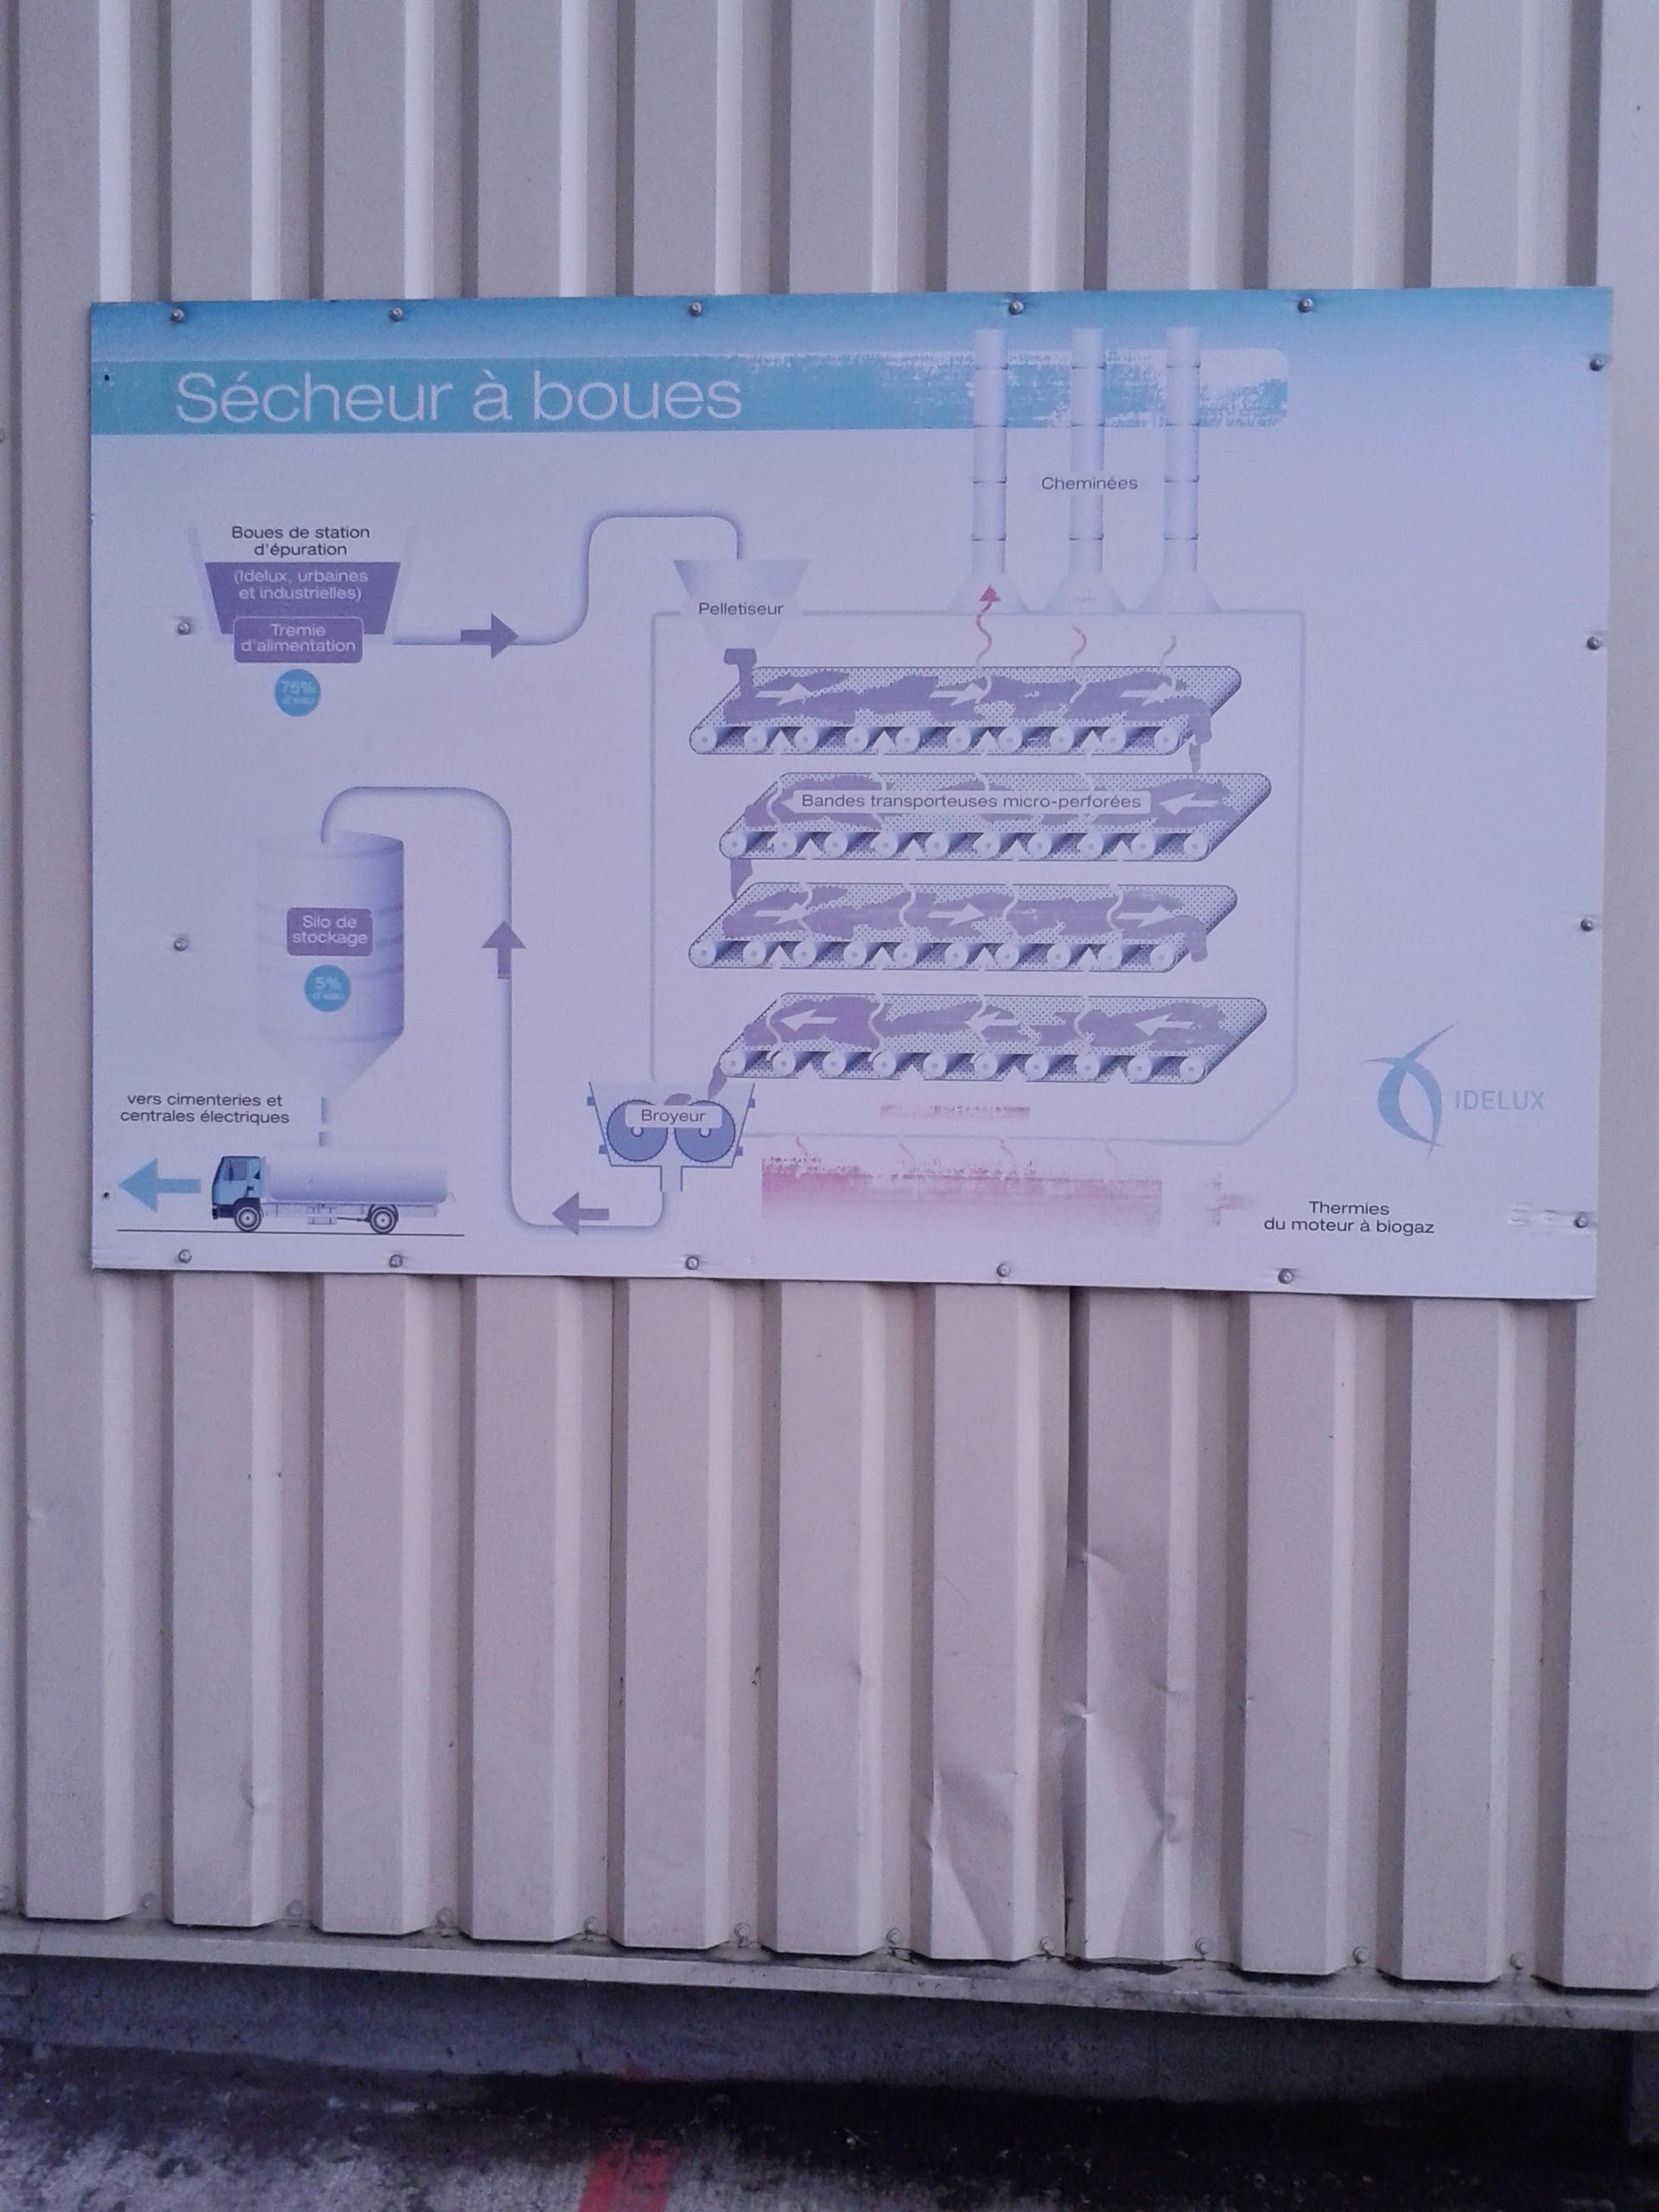
\includegraphics[scale=0.07]{task7/tenneville/IMG_20141105_113638.jpg}
  \caption{Sécheur à boue}
  \label{fig:Secheur}
\end{figure}
\subsubsection{Le compostage}
Le compostage se fait par bio-séchage de 2-3 semaines du digesta ainsi que de déchets verts. Pour ce faire, le mélange est placé sur des dalles où de l'air va circuler afin de garder un taux d'oxygène assez élevé tout en gardant une chaleur avoisinant les \unit{60}{\celsius}.
\begin{figure}
  \centering
  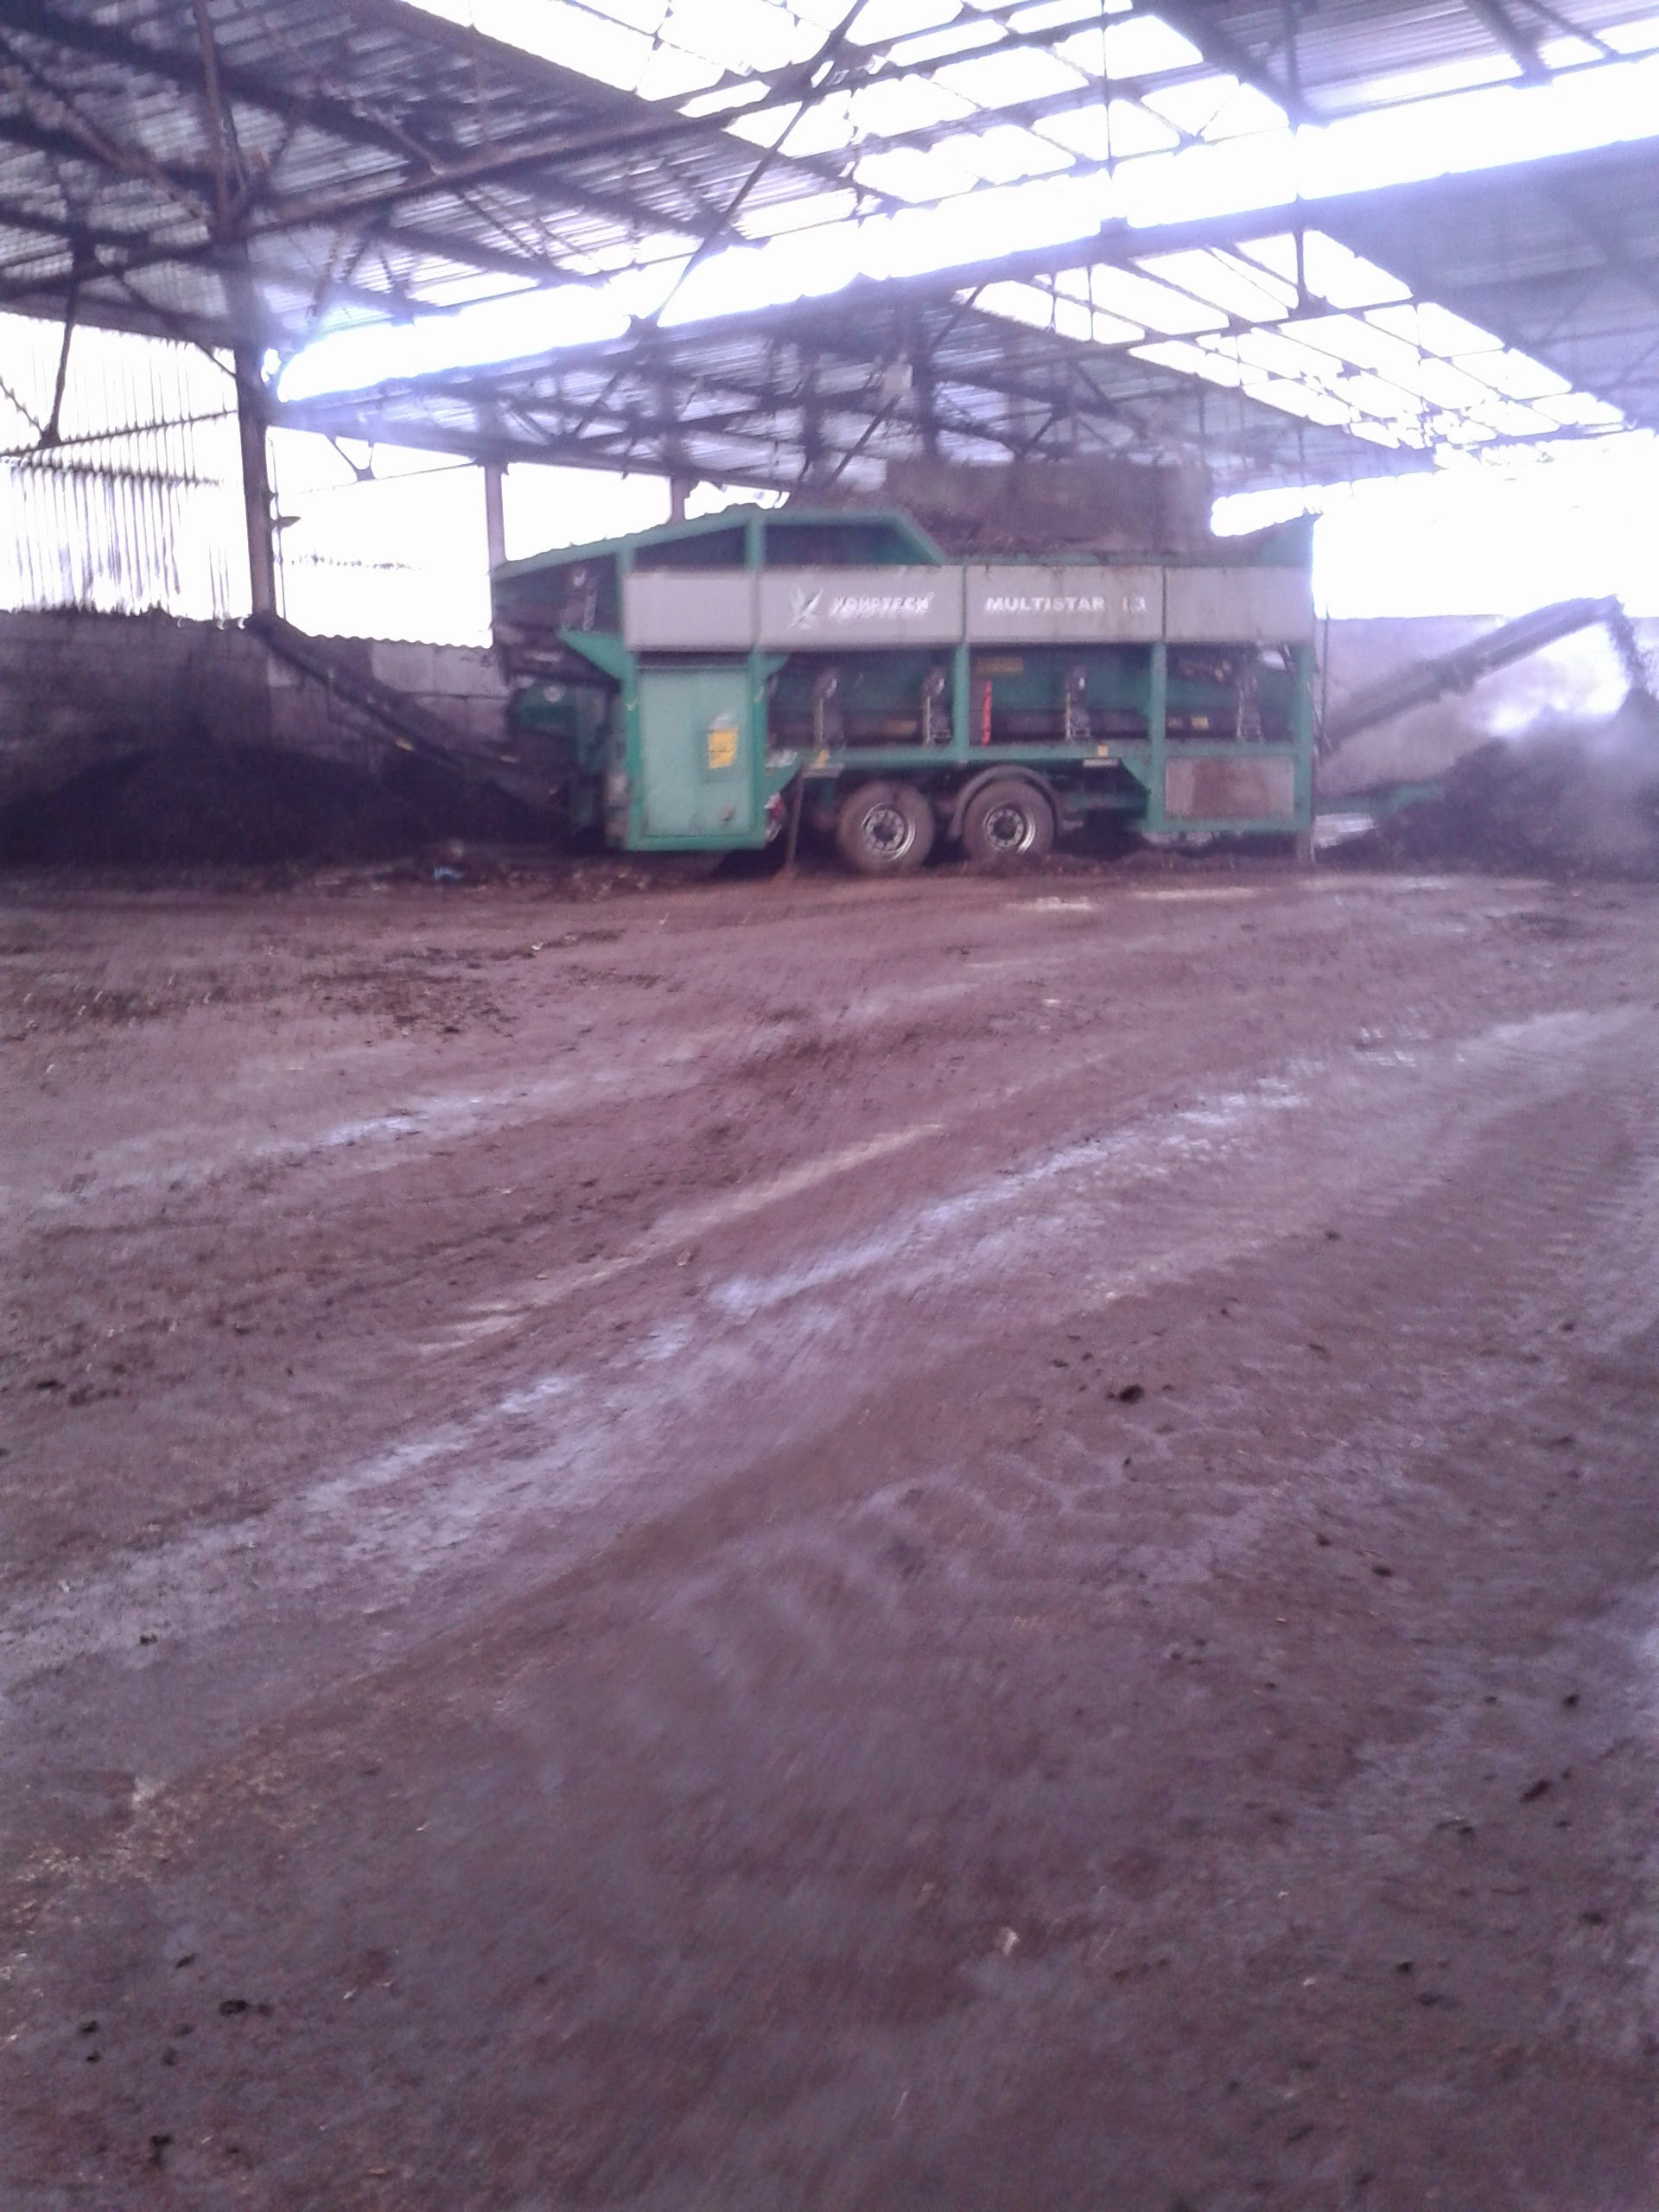
\includegraphics[scale=0.07]{task7/tenneville/IMG_20141105_102726.jpg}
  \caption{Tamiseur}
  \label{fig:tamiseur}
\end{figure}
Le mélange passe alors dans une machine à tamis (figure~\ref{fig:tamiseur}) qui le sépare en 3 tas:
\begin{enumerate}
\item Granulométrie $< \unit{12}{mm}$ (figure~\ref{fig:Granu12}).
\item Granulométrie $< \unit{20}{mm}$.
\item Granulométrie $> \unit{20}{mm}$ (figure~\ref{fig:granumore20}).
\end{enumerate}
\begin{figure}
  \centering
  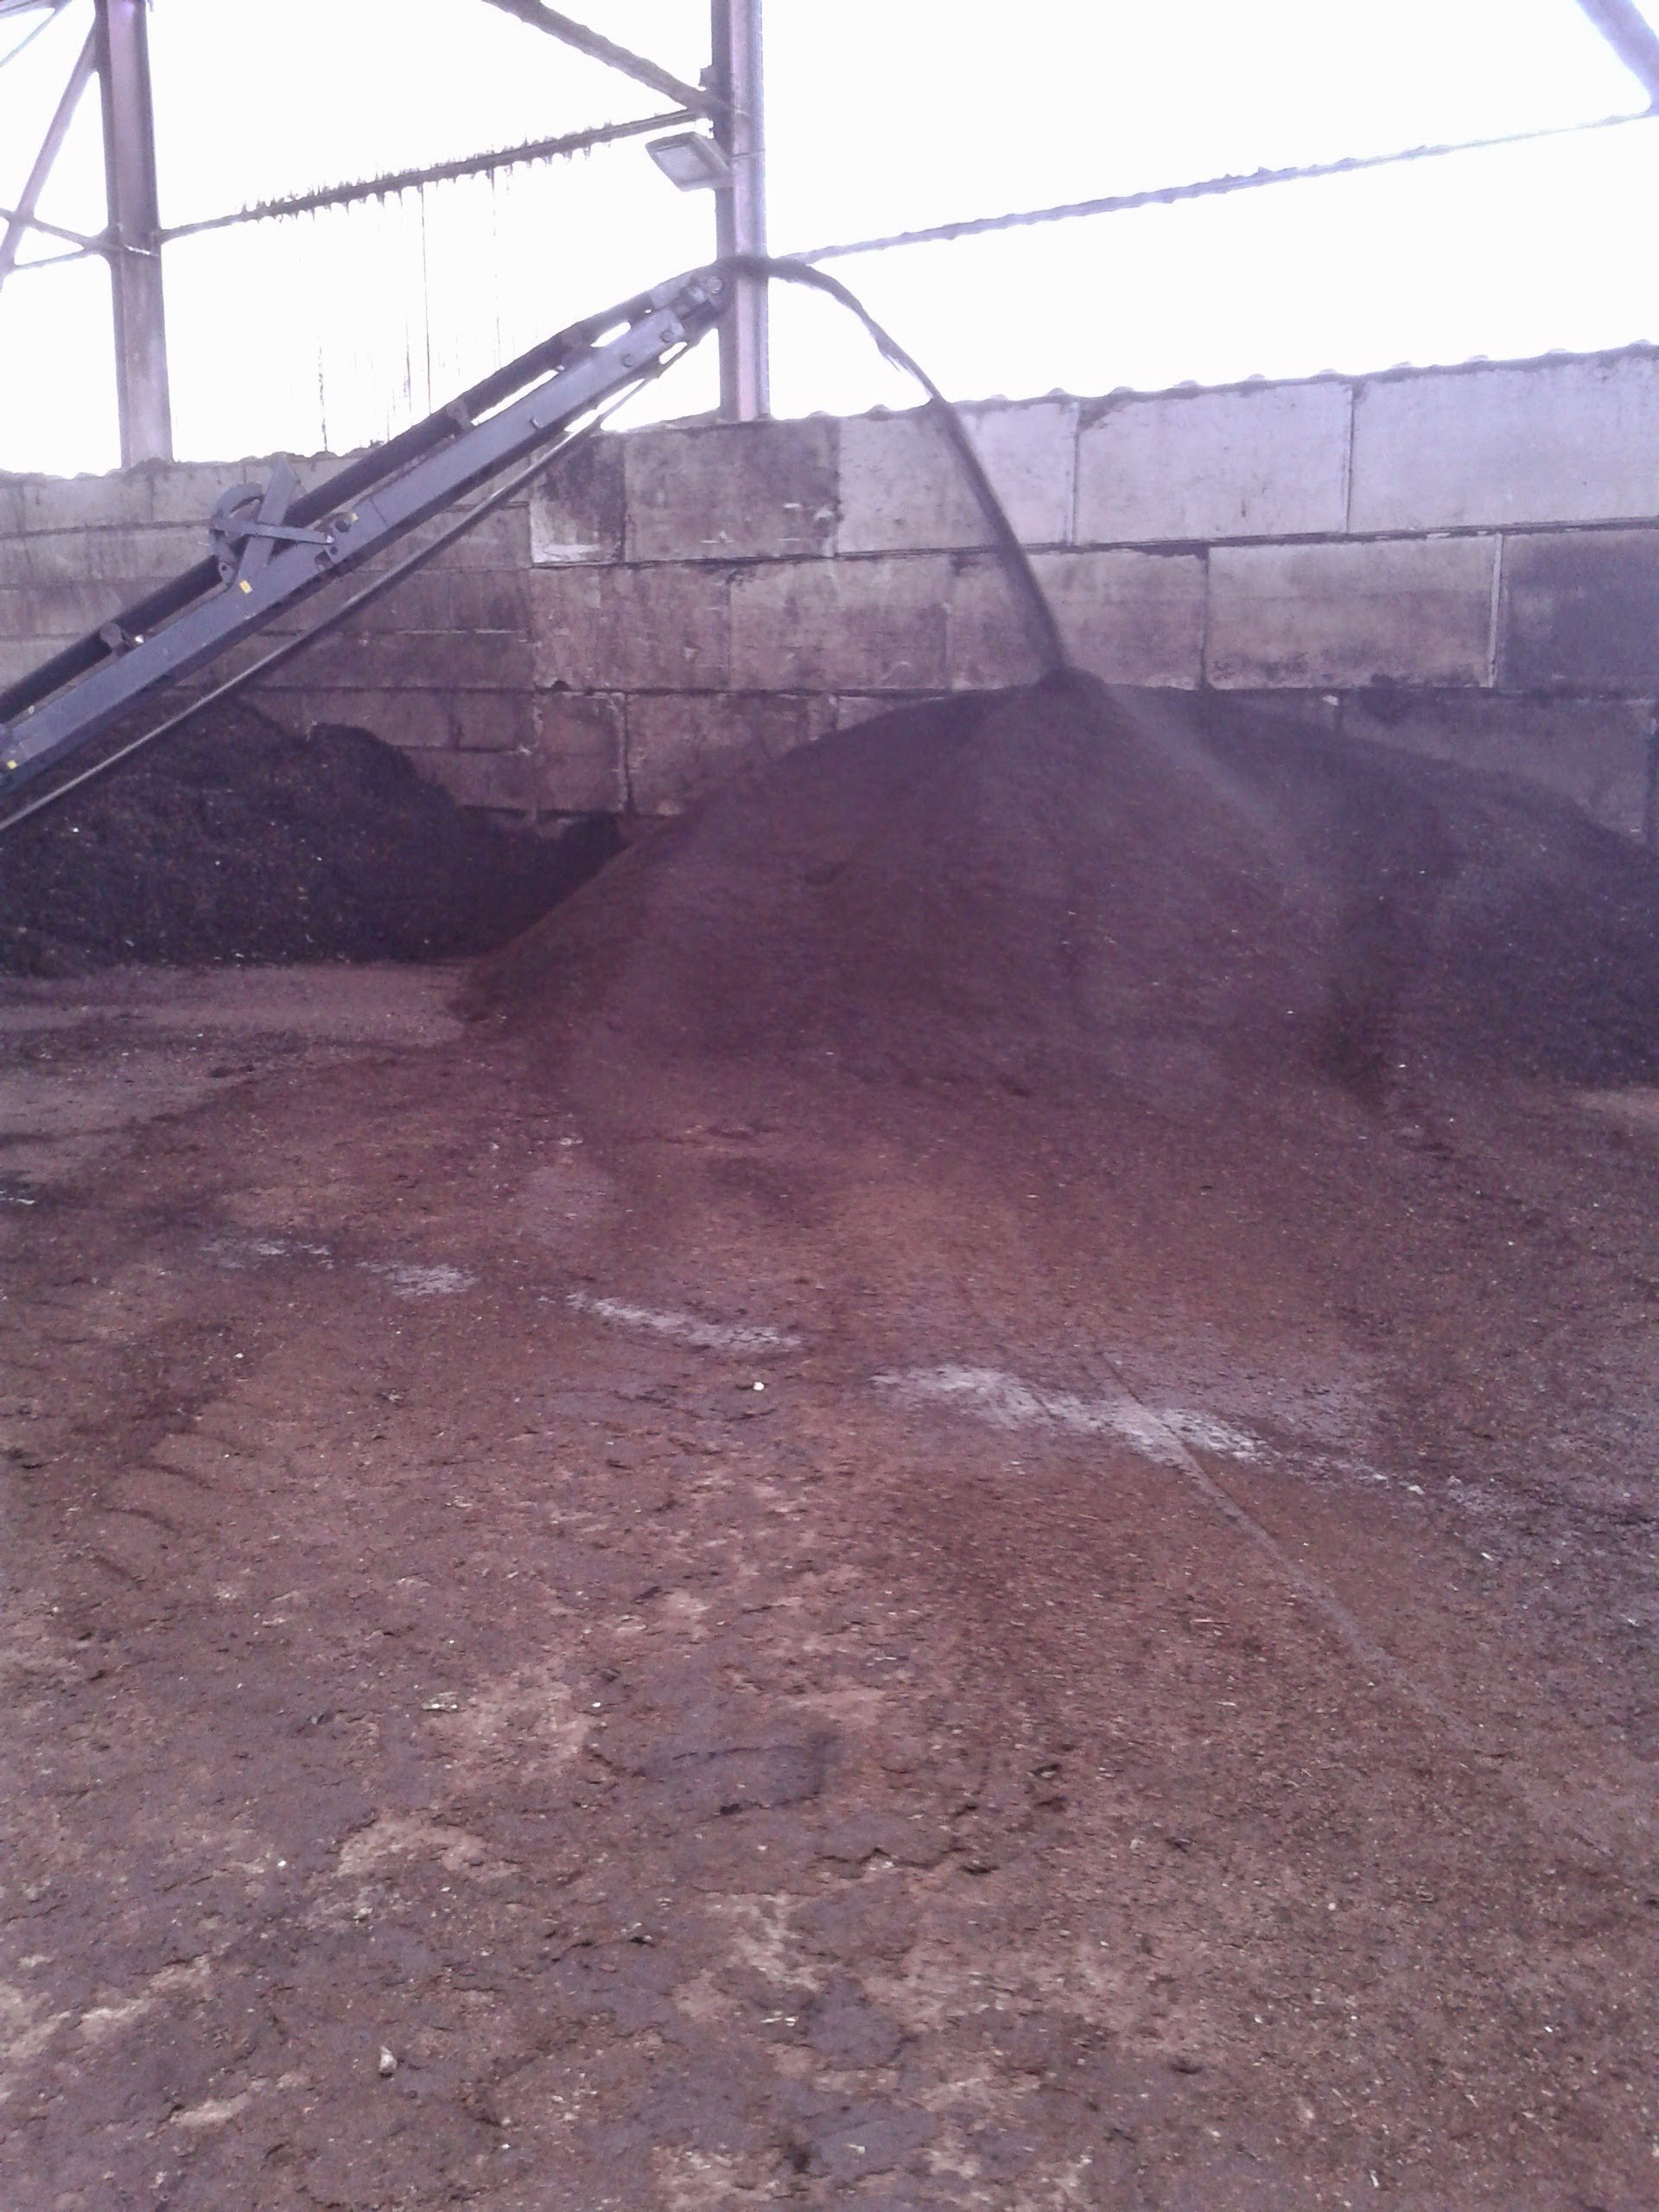
\includegraphics[scale=0.07]{task7/tenneville/IMG_20141105_103027.jpg}
  \caption{Granulométrie $< \unit{12}{mm}$}
  \label{fig:Granu12}
\end{figure}
\begin{figure}
  \centering
  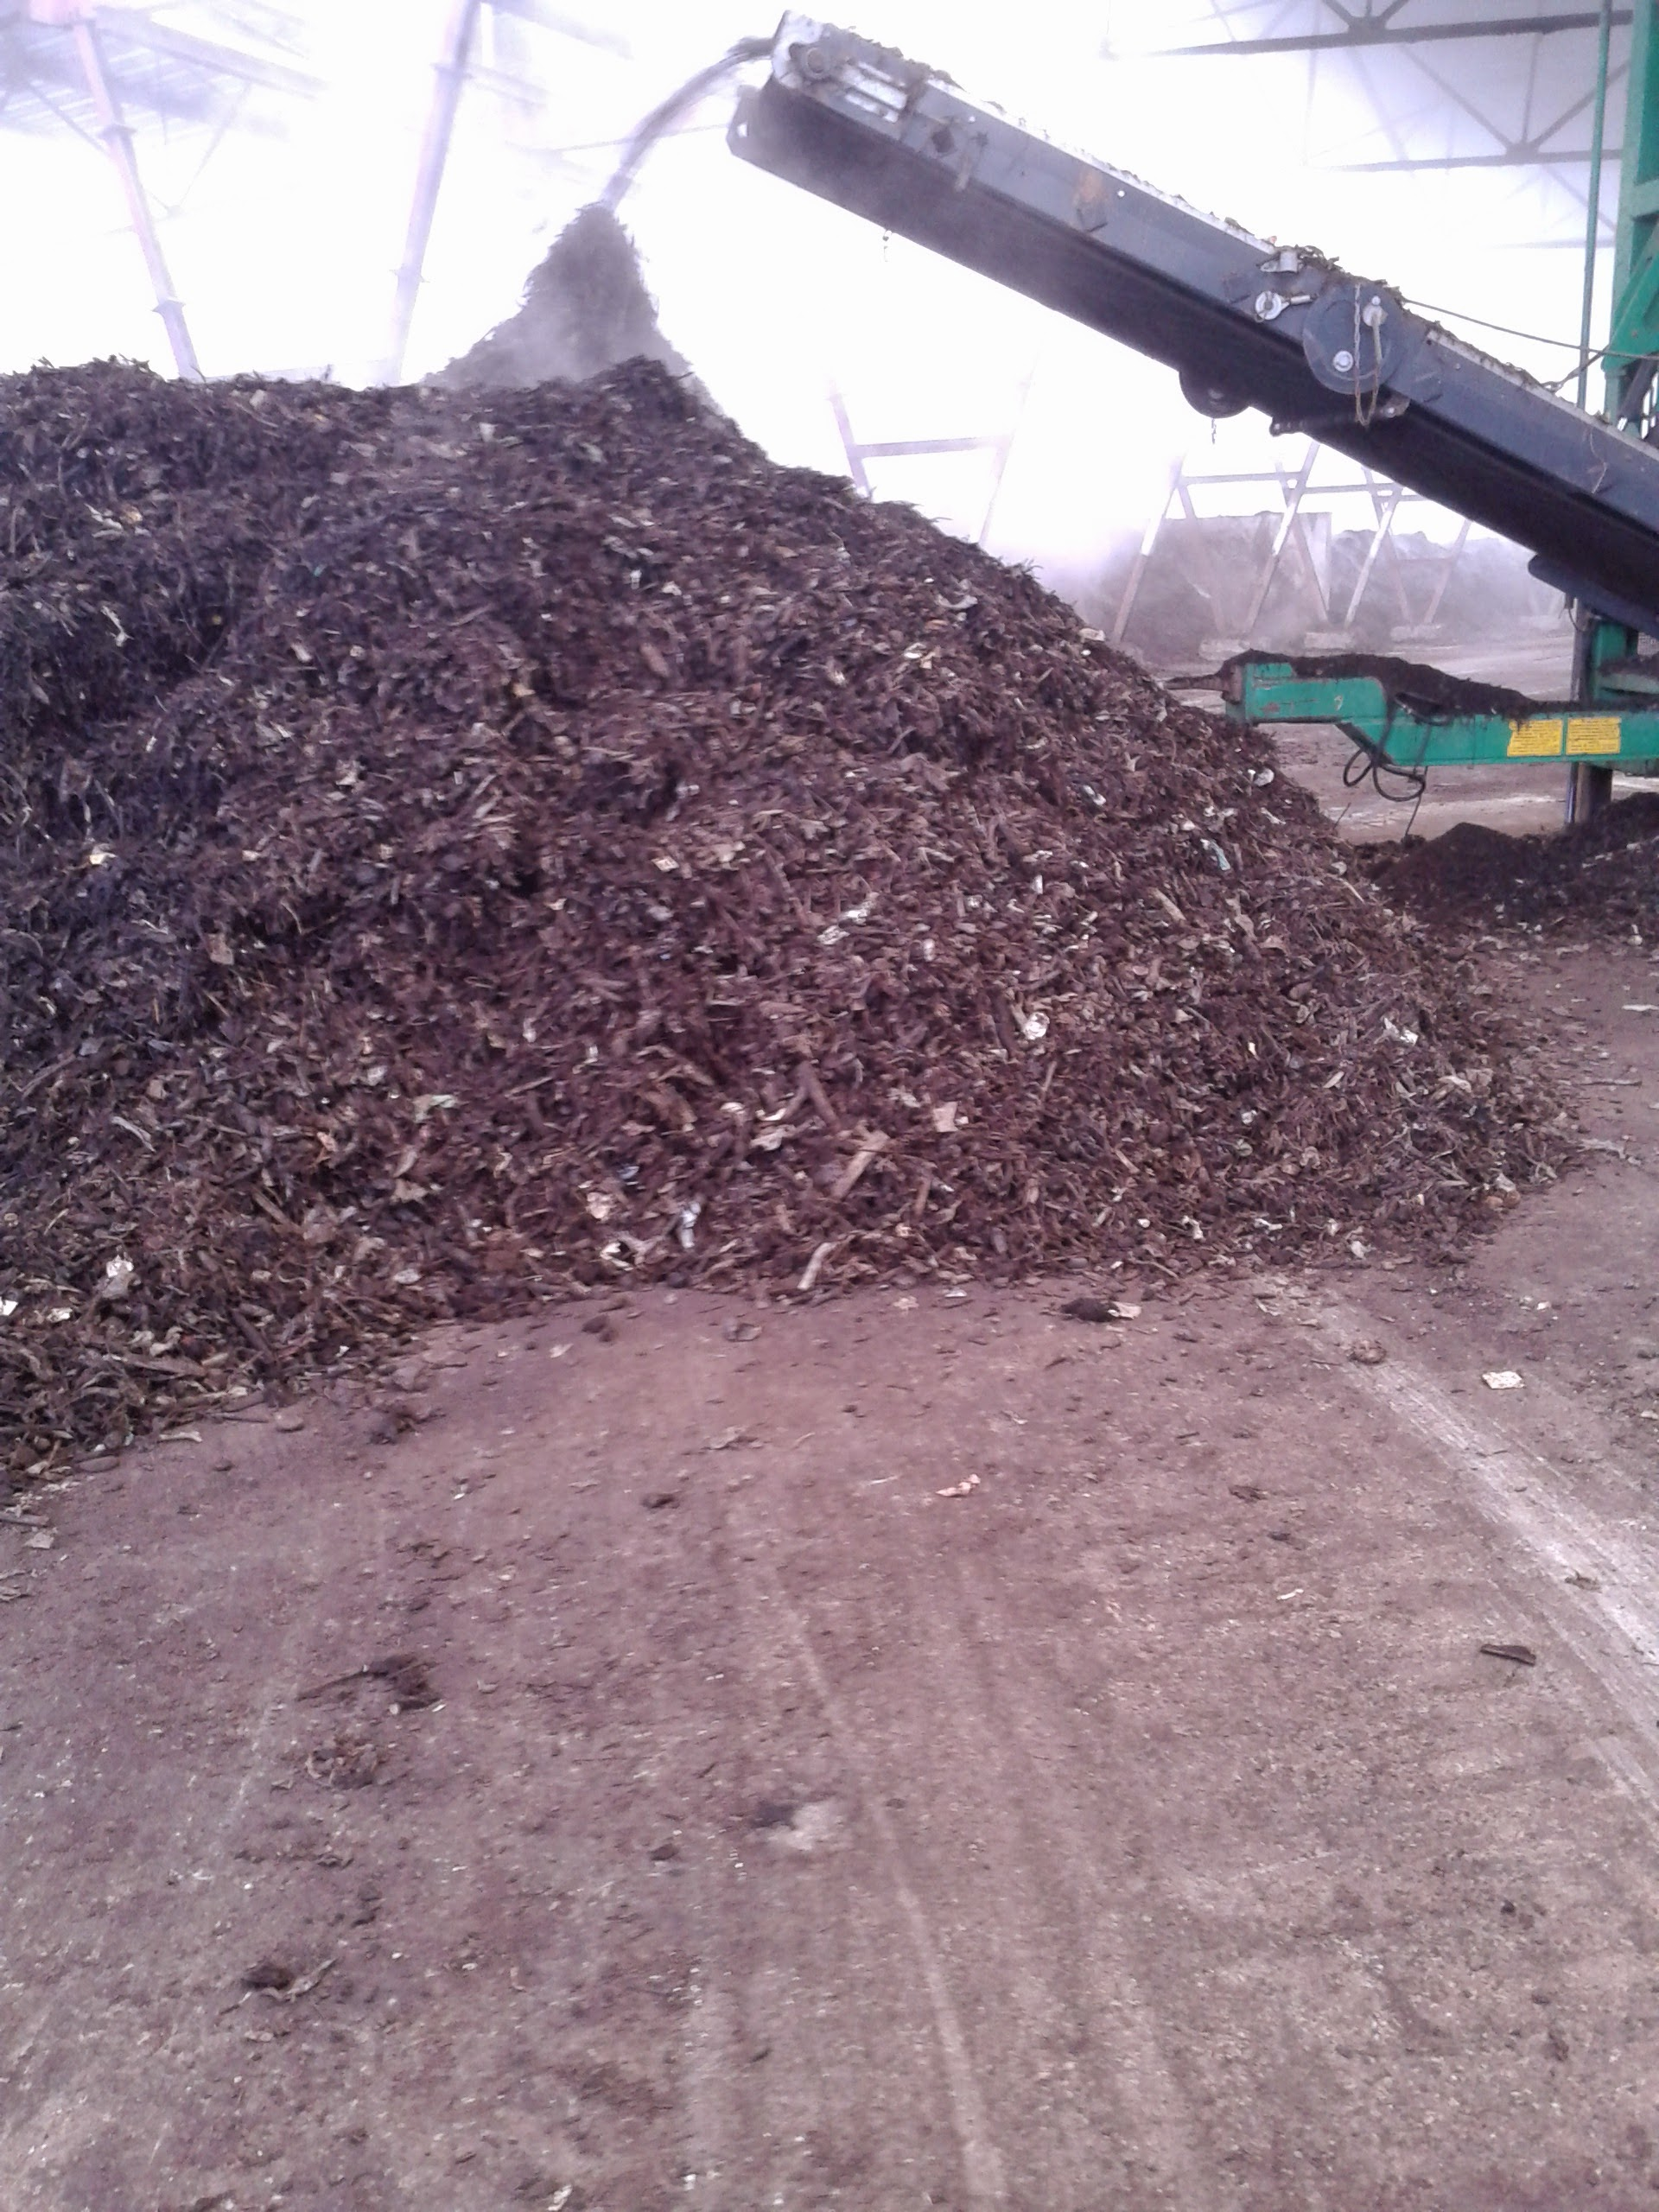
\includegraphics[scale=0.07]{task7/tenneville/IMG_20141105_103019.jpg}
  \caption{Granulométrie $> \unit{20}{mm}$}
  \label{fig:granumore20}
\end{figure}
La coupure avec une granulométrie supérieure à \unit{20}{mm} pourra être réinjectée dans le cycle tandis que celle avec une granulométrie inférieure à \unit{12}{mm} subira un traitement de maturation de 6 à 8 semaines afin d'être revendue 5 euro la tonne comme terreau.

En hiver, afin d'avoir une température suffisante, de la chaux vive sera ajoutée (le terreau pourra alors être vendu 8 euro la tonne).
\subsection{Conclusion}
Pour notre projet, il serait intéressant de se coupler avec une telle installation. En effet, celle-ci produit du méthane et de la chaleur tout en ayant un impact positif sur l'environnement.

Acheter le méthane qui transiterait via gazoduc, serait peut-être aussi à explorer bien que cette possibilité ne soit pas envisageable à Tenneville.